\documentclass[11pt,a4paper]{article}

\usepackage[T1]{fontenc}
\usepackage[utf8]{inputenc}
\usepackage[margin=2.5cm]{geometry}
\usepackage{graphicx}
\usepackage{booktabs}
\usepackage{xcolor}
\usepackage{tcolorbox}
\usepackage{enumitem}
\usepackage{float}
\usepackage[hidelinks]{hyperref}

% figures: works both inside the repo (results/figures/) and on Overleaf
% if the PNGs are uploaded into a folder called figures/
\graphicspath{{results/figures/}{figures/}}

% placeholder box for content still to be written
\newtcolorbox{placeholder}{colback=yellow!10, colframe=orange!70!black,
  boxrule=0.5pt, arc=2pt, left=4pt, right=4pt, top=2pt, bottom=2pt}

\setlist{itemsep=2pt, topsep=4pt}

\title{Benchmarking LLMs and VLMs for Automated De-Identification\\
of Clinical Text and Medical Images}
\author{Adnana Ivana \and Jiatong Li}
\date{}

\begin{document}
\maketitle

\section{Introduction}

Protected health information (PHI), such as names, dates, addresses and ID numbers, appears both in clinical text and burned into the pixels of medical images. We study whether one model family (Qwen) can find and remove PHI in both modalities. The project has two tracks:

\begin{itemize}
  \item \textbf{Text track} (Adnana Ivana): an LLM (Qwen3) finds PHI spans in synthetic clinical queries from ASQ-PHI.
  \item \textbf{Image track} (Jiatong Li): a VLM (Qwen3-VL) finds PHI in medical images from MIDI-B.
\end{itemize}

The task is information extraction, closely related to named entity recognition (NER): given a text, return every PHI span and its category. A missed PHI mention is a real privacy leak, so \textbf{recall is our primary metric}.

\begin{placeholder}
\textbf{[Image track: to be filled in by Jiatong.]}
\end{placeholder}

\section{Data set}

\paragraph{Text track: ASQ-PHI.} The file \texttt{ASQ/synthetic\_clinical\_queries.txt} contains synthetic clinical questions. Each query comes with its PHI tags, and each tag has an \texttt{identifier\_type} and the \texttt{value} as it appears in the text.

\begin{itemize}
  \item 1051 queries, 2973 gold PHI spans
  \item 219 queries contain no PHI at all, which lets us measure over-redaction
  \item 13 ASQ PHI types. The most frequent are GEOGRAPHIC\_LOCATION (826), NAME (814), DATE (806) and MEDICAL\_RECORD\_NUMBER (305). Several are very rare: ACCOUNT\_NUMBER (4), FAX\_NUMBER (2), CERTIFICATE\_LICENSE\_NUMBER (1) and IP\_ADDRESS (1).
\end{itemize}

\begin{placeholder}
\textbf{[Dataset source, construction and licence for ASQ-PHI: to be added.]}
\end{placeholder}

\paragraph{Shared taxonomy.} To compare the two tracks, both datasets are mapped onto five shared labels (Table~\ref{tab:taxonomy}).

\begin{table}[H]
\centering
\begin{tabular}{lp{0.55\textwidth}r}
\toprule
shared label & ASQ-PHI types & gold spans \\
\midrule
NAME     & NAME & 814 \\
DATE     & DATE & 806 \\
LOCATION & GEOGRAPHIC\_LOCATION & 826 \\
CONTACT  & phone, fax, email, IP address & 79 \\
ID       & medical record, health plan, SSN, unique ID, account, certificate/licence & 448 \\
\bottomrule
\end{tabular}
\caption{Shared PHI taxonomy and the number of ASQ-PHI gold spans per label.}
\label{tab:taxonomy}
\end{table}

The reviewers pointed out that a gap between the tracks might come from the datasets and not from the modality. The plan is to compare the tracks only on the shared categories that have enough support in \emph{both} datasets.

\begin{placeholder}
\textbf{[Image track: MIDI-B description, its mapping onto the shared taxonomy, licence, and which categories have enough support in both datasets.]}
\end{placeholder}

\section{Preprocessing}

ASQ-PHI gives the PHI values but not their positions in the text, so we compute character offsets ourselves:

\begin{itemize}
  \item \textbf{Gold spans:} each tagged value is located in its query by string search, and standalone matches (not inside a longer word) are preferred. Curly quotes are normalised. All gold values were found. One of them (\texttt{asq\_0149}, ``Children's Clinic'') matched only after quote normalisation.
  \item \textbf{Model output:} the LLM returns span strings, not offsets. Each string is aligned to the text with an exact match first and a normalised fuzzy match as a fallback. Strings that cannot be found are marked \emph{ungrounded} and count as false positives.
\end{itemize}

No other NLP preprocessing (tokenisation, lemmatisation, etc.) is applied. The models see the raw query.

\begin{placeholder}
\textbf{[Image track preprocessing.]}
\end{placeholder}

\section{Model training}

No model is trained. We compare prompting conditions of a pretrained LLM against an existing non-LLM tool.

\paragraph{LLM (Qwen3).} The current results are from \textbf{Qwen3-0.6B}, a small model used to test the pipeline. The proposal plans \textbf{Qwen3-8B}, and those runs are still to come. Setup:

\begin{itemize}
  \item non-thinking mode and greedy decoding
  \item \textbf{constrained JSON decoding} (\texttt{outlines} with a Pydantic schema), so every output is a valid list of \texttt{\{type, text\}} spans using the five shared labels
  \item two conditions:
  \begin{itemize}
    \item \textbf{zero-shot:} instructions only
    \item \textbf{few-shot:} the same instructions plus 3 hand-written examples (easy, tricky, and a hard negative with no PHI). The examples are not taken from ASQ-PHI, so no test data leaks into the prompt.
  \end{itemize}
  \item A third condition with Qwen3's ``thinking'' mode is planned but \textbf{has not been run yet}.
\end{itemize}

\paragraph{Non-LLM baseline: Microsoft Presidio.} The reviewers asked for a reference point beyond zero-shot vs few-shot. Presidio (\texttt{presidio-analyzer}) is an existing PII detector that combines spaCy NER (\texttt{en\_core\_web\_lg}) with rule-based recognizers. It runs with default settings and no score threshold. Its entity types are mapped onto the shared labels (e.g.\ PERSON $\rightarrow$ NAME, DATE\_TIME $\rightarrow$ DATE, PHONE\_NUMBER/EMAIL\_ADDRESS/IP\_ADDRESS $\rightarrow$ CONTACT, US\_SSN/MEDICAL\_LICENSE/\ldots{} $\rightarrow$ ID).

All three conditions write the same prediction format and are scored by the same code.

\begin{placeholder}
\textbf{[Image track: Qwen3-VL setup.]}
\end{placeholder}

\section{Evaluation}

\paragraph{Metrics.} Each predicted span is compared with the gold spans of the same query in three modes (Table~\ref{tab:modes}).

\begin{table}[H]
\centering
\begin{tabular}{lp{0.7\textwidth}}
\toprule
mode & a prediction counts as correct if\ldots \\
\midrule
strict  & same start, end and label \\
overlap & the characters overlap and the label is the same \\
any     & the characters overlap, label ignored. This is the privacy view: \emph{would this PHI have been redacted?} \\
\bottomrule
\end{tabular}
\caption{Matching modes.}
\label{tab:modes}
\end{table}

We report micro-averaged precision, recall and F1, overall, per shared category and per ASQ type. At the query level we report:

\begin{itemize}
  \item \textbf{leak-free rate:} the share of queries with PHI where every gold span was caught (any mode)
  \item \textbf{false-alarm rate:} the share of queries \emph{without} PHI where something was still flagged
\end{itemize}

Results below are for all 1051 queries.

\paragraph{Overall.} Table~\ref{tab:overall} shows the scores in overlap mode, and Figure~\ref{fig:overall} shows all three modes.

\begin{table}[H]
\centering
\begin{tabular}{lccc}
\toprule
condition & precision & recall & F1 \\
\midrule
Qwen3-0.6B zero-shot & 0.726 & 0.285 & 0.409 \\
Qwen3-0.6B few-shot  & 0.869 & 0.427 & 0.573 \\
Presidio             & 0.620 & \textbf{0.767} & \textbf{0.686} \\
\bottomrule
\end{tabular}
\caption{Overall micro-averaged scores, overlap mode.}
\label{tab:overall}
\end{table}

\begin{figure}[H]
\centering
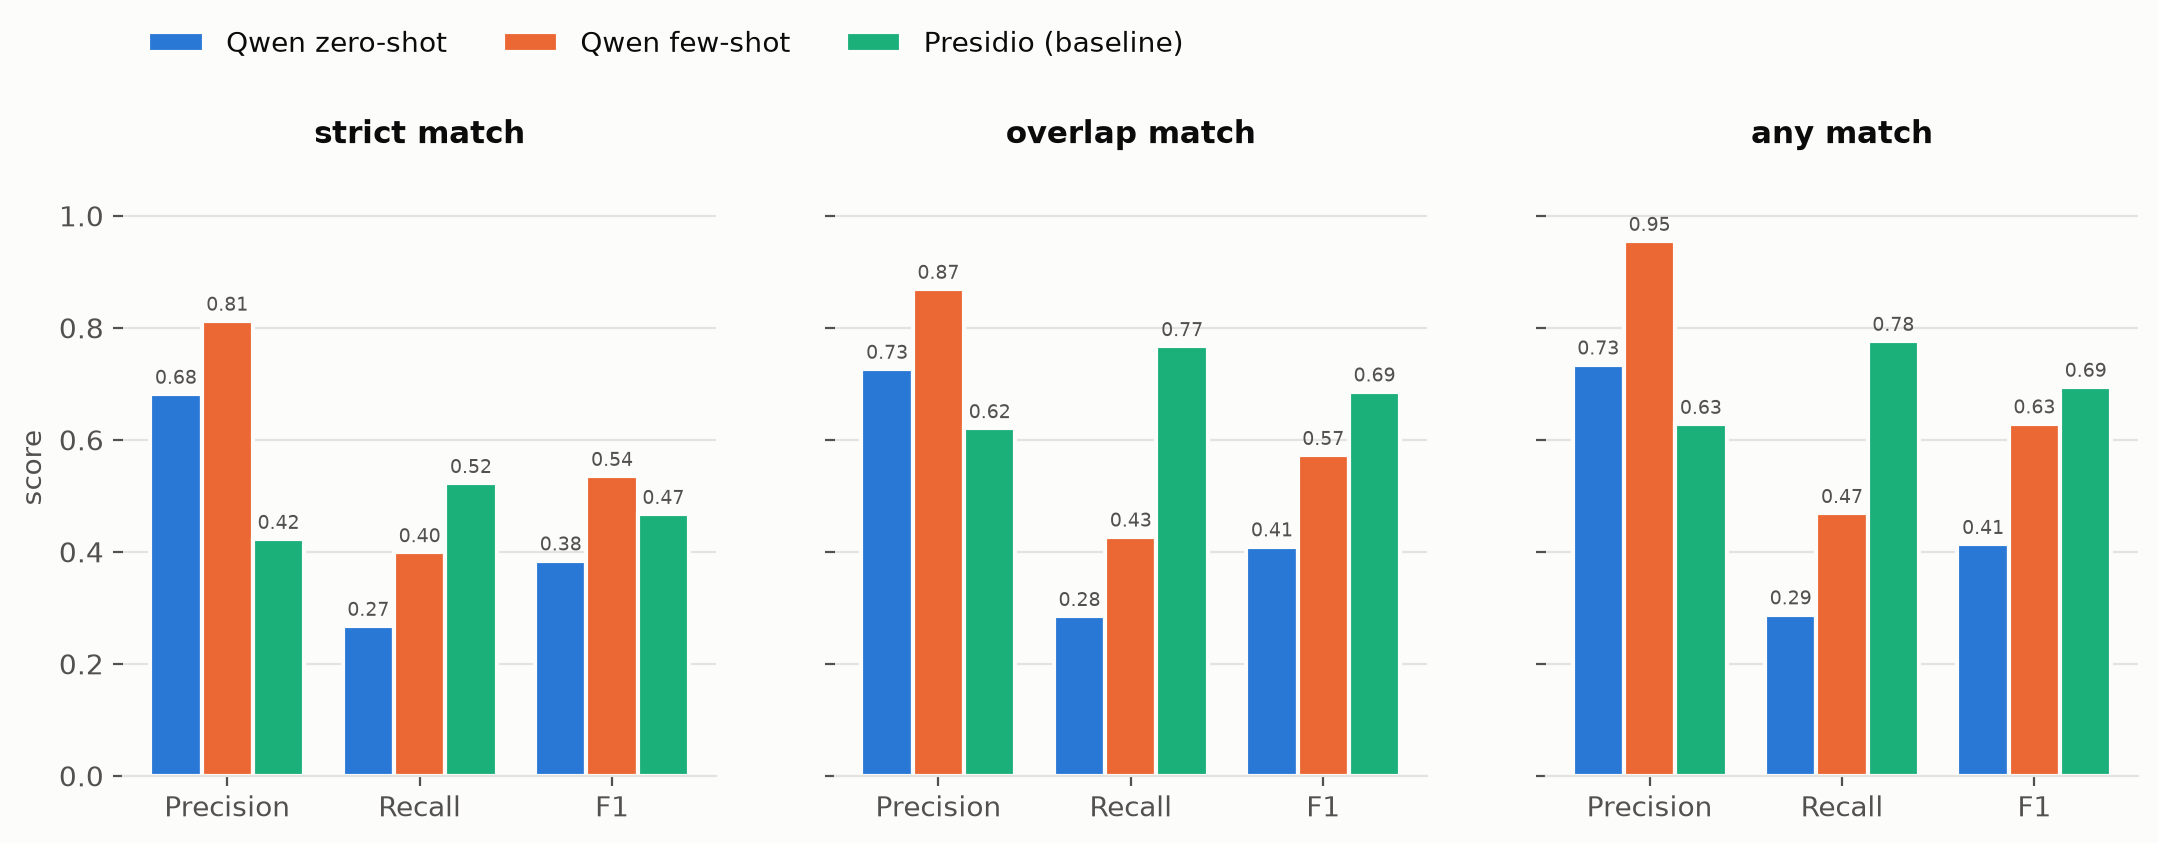
\includegraphics[width=\textwidth]{qwen3-0.6b_overall.png}
\caption{Overall precision, recall and F1 in the three matching modes.}
\label{fig:overall}
\end{figure}

\begin{itemize}
  \item \textbf{Few-shot examples help the small LLM a lot.} Recall rises from 0.29 to 0.43 and precision from 0.73 to 0.87. The share of ungrounded spans (strings not found in the query) drops from 23.1\% to 1.3\%.
  \item \textbf{Presidio has much higher recall than Qwen3-0.6B} (0.77 vs 0.43) but lower precision. With recall as the main metric, the baseline currently wins.
\end{itemize}

\paragraph{Per category.} Figure~\ref{fig:category} shows recall and precision per shared category.

\begin{figure}[H]
\centering
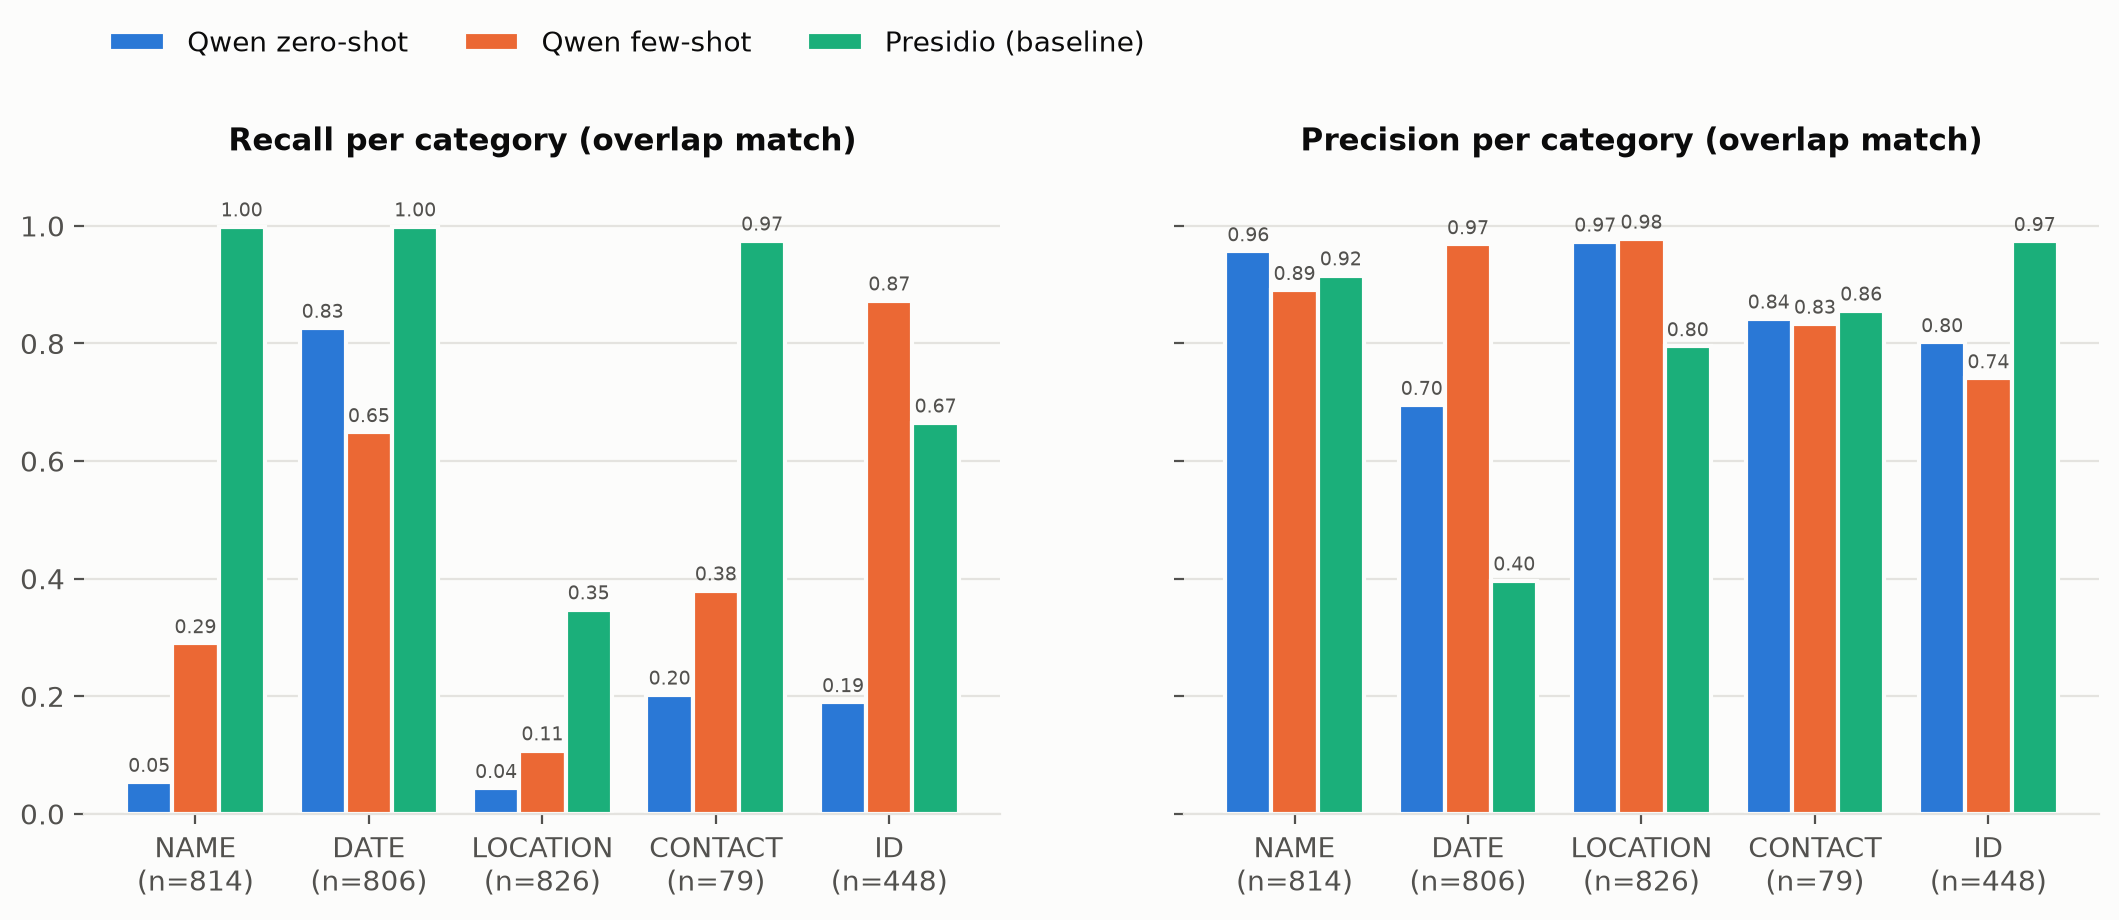
\includegraphics[width=\textwidth]{qwen3-0.6b_per_category.png}
\caption{Recall and precision per shared category (overlap mode).}
\label{fig:category}
\end{figure}

\begin{itemize}
  \item \textbf{Presidio} finds almost all names, dates and contact details (recall 1.00, 1.00 and 0.97). Its DATE precision is only 0.40, because it also tags ages (``60-year-old'') and years on their own (``2023''), which ASQ-PHI does not annotate as PHI.
  \item \textbf{Few-shot Qwen is better on IDs} (recall 0.87 vs 0.67 for Presidio). This holds for medical record numbers in particular (any mode: 0.92 vs 0.70) and social security numbers (0.67 vs 0.36).
  \item \textbf{LOCATION is hard for every condition} (recall 0.04 / 0.11 / 0.35), and it is the largest category (826 spans).
  \item \textbf{The few-shot LLM is weak on names} (recall 0.29), and zero-shot even more so (0.05).
  \item Zero-shot DATE recall (0.83) is higher than few-shot (0.65). The few-shot examples do not help every category.
\end{itemize}

\paragraph{Query level.} Figure~\ref{fig:query} shows the leak-free and false-alarm rates.

\begin{figure}[H]
\centering
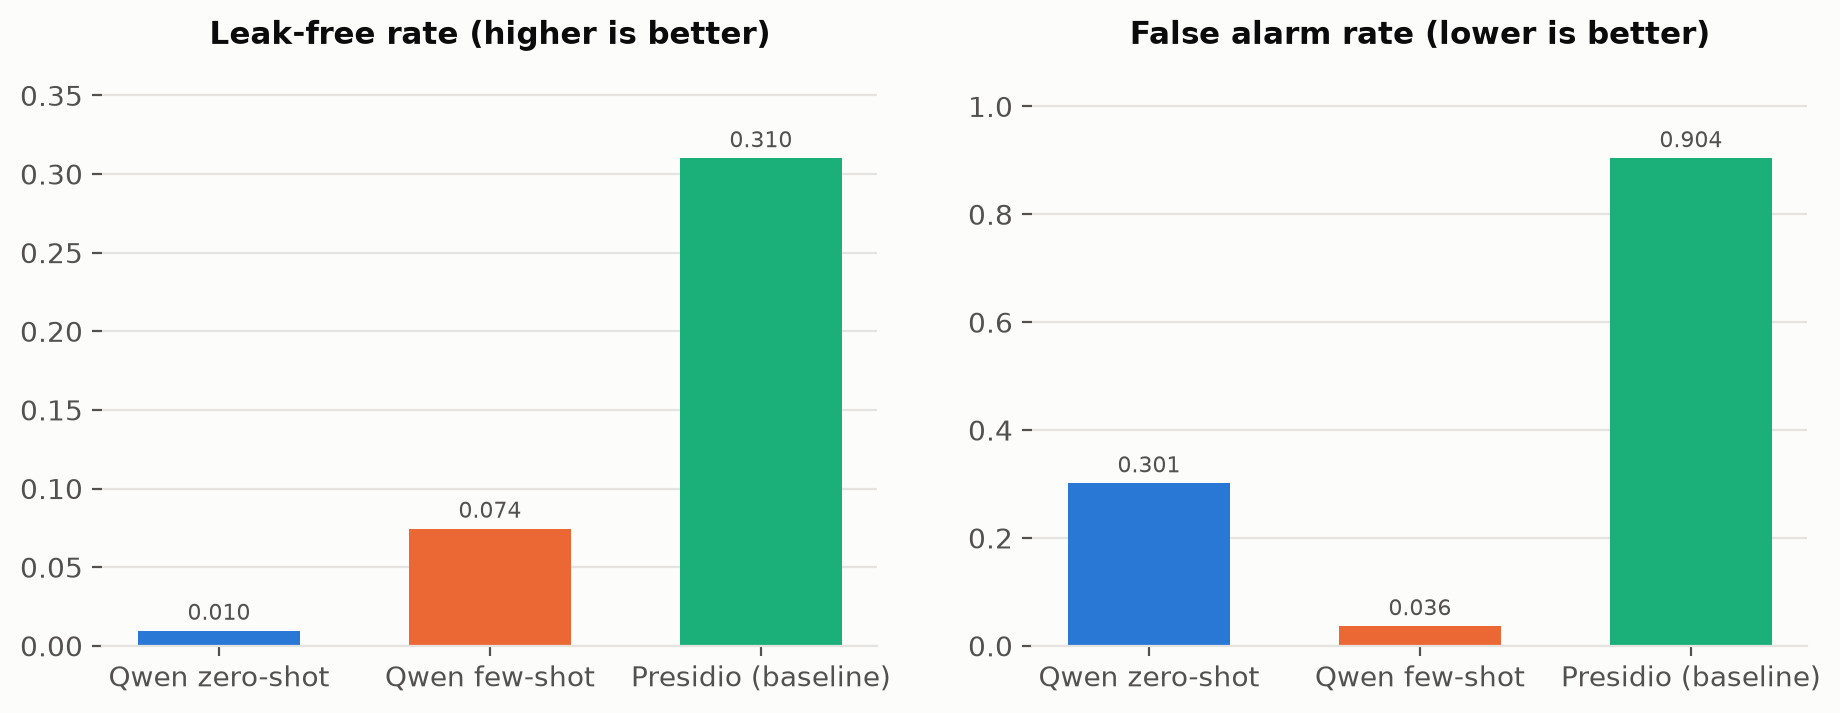
\includegraphics[width=0.9\textwidth]{qwen3-0.6b_query_level.png}
\caption{Leak-free rate and false-alarm rate.}
\label{fig:query}
\end{figure}

\begin{itemize}
  \item No condition fully de-identifies most queries. The leak-free rate is 0.010 for zero-shot, 0.074 for few-shot and 0.310 for Presidio.
  \item Presidio over-redacts heavily: it flags something in 90\% of the queries that contain no PHI. For few-shot Qwen this is 3.7\%.
\end{itemize}

\paragraph{Main outcome so far.} The small Qwen3-0.6B model is precise but misses most PHI. An off-the-shelf tool (Presidio) catches much more, at the cost of many false alarms. Few-shot prompting clearly improves the LLM. Whether a larger model (Qwen3-8B) closes the recall gap is still open.

More figures (e.g.\ recall per ASQ type) are in \texttt{results/figures/}, and all numbers are in \texttt{results/*.csv}.

\begin{placeholder}
\textbf{[Image track: evaluation and results on MIDI-B.]}\\[4pt]
\textbf{[Cross-modality comparison on the shared categories.]}
\end{placeholder}

\section{Future work}

\begin{itemize}
  \item Run the planned \textbf{Qwen3-8B} model and the \textbf{thinking} condition on the full dataset.
  \item Look at the remaining errors more closely, especially missed locations and names, and the boundary and label mistakes.
  \item Make the comparison with Presidio fairer, e.g.\ by testing a score threshold or excluding ages and bare years. Its default settings trade precision for recall.
  \item Complete the cross-modality comparison with the image track on the shared categories.
\end{itemize}

\begin{placeholder}
\textbf{[Image track: future work.]}
\end{placeholder}

\end{document}
